\documentclass{article}
\usepackage[T1]{fontenc}
\usepackage{lmodern}
\usepackage{graphicx}
\usepackage{amsmath,amssymb}
\usepackage[a4paper,margin=2cm]{geometry}
\usepackage[absolute,overlay]{textpos}
\setlength{\TPHorizModule}{1mm}
\setlength{\TPVertModule}{1mm}
\usepackage[indonesian]{babel}
\usepackage{hyperref}
\setlength{\emergencystretch}{2em}
% unit: Halaman 13

\begin{document}

% === Halaman 13 (llm) ===

\bullet Contoh lain:

\vspace{197.21mm}

\begin{align*}
 m &= (y_p - y_q)/(x_p - x_q) \\
 &= (-1.86 - 0.836)/(-2.35 - (-0.1)) \\
 &= -2.696 / -2.25 = 1.198 
\end{align*}

\begin{align*}
 x_r &= m^2 - x_p - x_q \\
 &= (1.198)^2 - (-2.35) - (-0.1) \\
 &= 3.89 
\end{align*}

\begin{align*}
 y_r &= m(x_p - x_r) - y_p \\
 &= 1.198(-2.35 - 3.89) - (-1.86) \\
 &= -5.62 
\end{align*}

\vspace{10mm}

Sumber gambar: Debdeep Mukhopadhyay, Elliptic Curve Cryptography, Dept of Computer Sc Engg IIT Madras

% deskripsi: Grafik kurva eliptik $y^2 = x^3 - 7x$ yang menunjukkan operasi penjumlahan titik $P + Q = R$, lengkap dengan garis bantu dan koordinat titik P, Q, R, dan -R.
% bbox normalisasi: [0.5050, 0.1260, 0.9200, 0.7900]
\begin{textblock*}{87.15mm}(106.05mm,37.42mm)
\noindent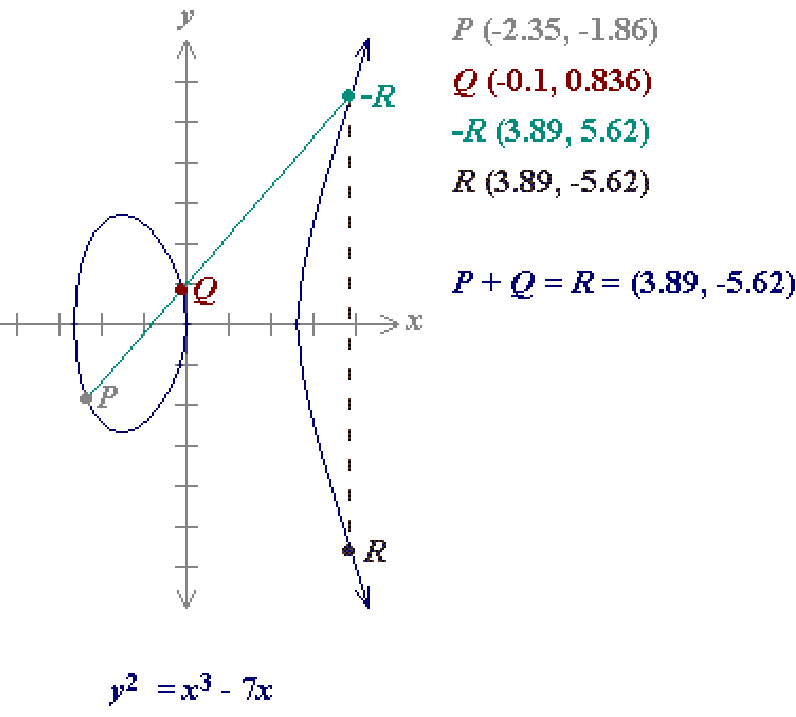
\includegraphics[width=87.15mm,height=197.21mm]{../../images/llm/page_013_img_01.png}%
\end{textblock*}

\end{document}
